% Im Theorieteil ist der aktuelle Stand der Technik/Forschung wertungsfrei darzustellen. Er dient dazu, den wissenschaftlichen Kontext für die Aufgabenstellung herauszuarbeiten. Dementsprechend sollte die Darstellungsweise nicht zu allgemein gewählt werden, sondern nur die für die Aufgabenstellung relevanten Theorien und notwendigen Definitionen dargelegt werden. Stehen mehrere Theorien zur Verfügung, ist ein Überblick zu geben. Definitionen sind nur dann notwendig, wenn sie nicht ohnehin als allgemein, d.h. von Vertreter des Fachbereichs, bekannt vorausgesetzt werden können und für den weiteren Verlauf der Arbeit relevant sind. Die Theorie hat einen entscheidenden Einfluss auf die Methodenwahl und die Interpretation der Ergebnisse. Der Stand der Technik ist u.a. dokumentiert in Monografien, Vortragsmanuskripten, Patenten und in besonderer Weise in Artikeln wissenschaftlicher Zeitschriften. Diese Quellen Seite 5 sind zu nutzen. Es wird eine Analyse von mindestens vier Zeitschriftenartikeln erwartet, von denen mindestens einer in englischer Sprache verfasst ist. Bei der Auswahl der Literatur ist auf Aktualität der Arbeiten zu achten.
\chapter{Theorie}
\section{Theorie zur Auslegung der künstlichen Muskeln}
Um die Baugruppe an die Bewegungen eines Billiardspielers anzupassen, müssen die Bauteile entsprechend ausgelegt werden. 
Dazu zählt unter anderem die Auslegung der Kraft der künstlichen Muskeln. 
Um dies richtig erfassen zu können wurde ein schematischer Aufbau des Arms angenommen und daran die Berechnungen ausgeführt. 
Zunächst allerdings wird der Impuls, den der Billiardqueue auf die Spielkugel überträgt betrachtet. 
Dabei gilt, dass die beiden Impulse bei unterschiedlicher Masse und Geschwindigkeiten identisch sind. 
\begin{equation}
	m_{Arm} \cdot v_{Arm} = m_{Kugel} \cdot v_{Kugel}
	\label{eq:ImpulsKugel}
\end{equation}
Dabei ist die Masse des Arms \(m_{Arm}\), die Bewegungsgeschwindigkeit des Arms \(v_{Arm}\), die Masse der Kugel \(m_{Kugel}\) und die Bewegungsgeschwindigkeit der Kugel \(v_{Kugel}\).
Damit kann die benötigte Bewegungsgeschwindigkeit an der Hand des Armes berechnet werden.
\begin{equation}
	v_{Arm} = \frac{m_{Kugel} \cdot v_{Kugel}}{m_{Arm}}
	\label{eq:SollgeschwindikeitArm}
\end{equation}

Die kann dann dazu genutzt werden die erforderliche Kraft der pneumatischen Muskeln zu berechnen.
Sie ist im folgenden mit \(v\) für die Sollgeschwindigkeit bezeichnet. \par
Nun wird über das Drehmoment die benötigte Kraft der künstlichen Muskeln oder auch PAMs berechnet. 



\begin{equation}
	M = b \cdot F = I \cdot \alpha
	\label{eq:DrehmomentArm}
	\end{equation}
	
	mit dem Trägheitsmoment \( I = m \cdot s_m^2 \), der Tangentialbeschleunigung \( a_T = \frac{v^2}{\Delta x} \) und der
	Winkelbeschleunigung \( \alpha = \frac{a_T}{B} \) \par\medskip
	
	\begin{align}
	I \cdot \frac{a_T}{B} &= m \cdot s_m^2 \cdot \frac{a_T}{B} \nonumber\\
	b \cdot F &= m \cdot s_m^2 \cdot \frac{a_T}{B} \nonumber\\
	F &=\frac{m \cdot {s_m}^2 \cdot a_T}{B \cdot b \cdot cos(\beta)}
	\label{eq:Kraft-PAM}
	\end{align}

	Eine Skizze zur Veranschaulichung, sowie die Beschreibungen der Variablen befinden sich auf der nächsten Seite. 
	
	\newpage
	\begin{figure}[h]
		\centering
		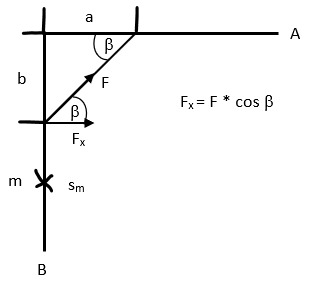
\includegraphics[width=.5\textwidth]{Abb/SkizzeBerechnungen.jpeg}
		\caption{Skizze Berechnungen.}
		\label{fig:SkizzeBerechnungen}
	\end{figure}

	hier sind
	
	\( m := \) Masse Unterarm \\
	\( s_m := \) Massenschwerpunkt entlang $ B $ \\
	\( v := \) Soll-Endgeschwindigkeit \\
	\( \Delta x := \) Ausholstrecke vor dem Stoß \\
	\( B := \) Strecke Drehachse - Ende des Unterarms \\
	\( b:= \) Strecke Drehachse - Angriffspunkt PAM \\
	\( \beta := \) Winkel PAM  Oberarm \\
	\( F:= \) Erforderliche Kraft des PAM

	\section{Theorie zur Auslegung des Schultergetriebes}
	Um den Queue korrekt anlegen zu können ist es erforderlich, dass sämtliche Unterbaugruppen vor, während und nach eines Stoßes in der eingestellten Ausrichtung verharren.
	Weiter muss die angestrebte Position an der Kugel, sowie der Stoßwinkel in ausreichender Präzision sicher angefahren werden können.
	Diese Aufgabe muss primär vom Schultergelenk geleistet werden, welches wie oben beschrieben mit einem Zykloidalgetriebe als Kernkomponente umgesetzt werden soll.
	Die Untersetzung \(N\) eines Zykloidalgetriebes lässt sich allgemein durch \cref{eq:untersetzung} darstellen.

	\begin{equation}
		N = -\frac{Z_2}{Z_1 - Z_2}
		\label{eq:untersetzung}
	\end{equation}

	Hier seien \(Z_1\) die Anzahl der Zähne der inneren Scheibe und \(Z_2\) die Anzahl der Zähne des einschließenden, äußeren Ringes.
	Aus der Geometrie geht zwingend hervor, dass \(Z_1 < Z_2\) gilt.
	Weiter kann mit dem Zusammenhang \(Z_2 - Z_1 = 1\) das Verhältnis von Untersetzungsvermögen zu räumlichen Volumen maximiert werden.
	Mit diesen Randbedingungen wird \cref{eq:untersetzung} zu \(N = Z_2\) und das Untersetzungsvermögen lässt sich somit unmittelbar an der Anzahl der Zähne des äußeren Ringes ablesen.\par\medskip